\section{Backgrounds}
\label{sect:bkg}
We separate the backgrounds into two categories.  Those with 
``fake'' \Tau, i.e., events where a quark or gluon jet has been misidentified
as a \Tau, and those without \Tau misidentifications.  
The fake \Tau backgrounds arise mostly from QCD and \wjets events.  The 
other backgrounds are from \ttbar, $Z+$ jets, diboson events as well as the Higgs boson decays.
Backgrounds with fake \Tau are mainly estimated with data-driven methods; the 
remaining backgrounds are taken from Monte Carlo events. The main backgrounds
are discussed here, but the others are very small, so they are dropped from the 
discussion.

\subsection{\texorpdfstring{QCD background estimation in the $\tauTau$ channel}{QCD background estimation in the tau-tau channel}}
\label{sect:bkgQCD}
Events from QCD jet production can enter the signal regions if two quark or gluon jets are 
misidentified as \Tau, and the rest of the kinematical selections are also 
satisfied.  
Isolation is an important 
discriminant between fake and real \Tau objects. For this purpose, the control regions are defined using the isolation variables for the \Tau 
pair and \mttwo or \SumMT, as illustrated in Fig.~\ref{fig:ABCDQCD}. 
\begin{figure}[!Hhtb]
\centering
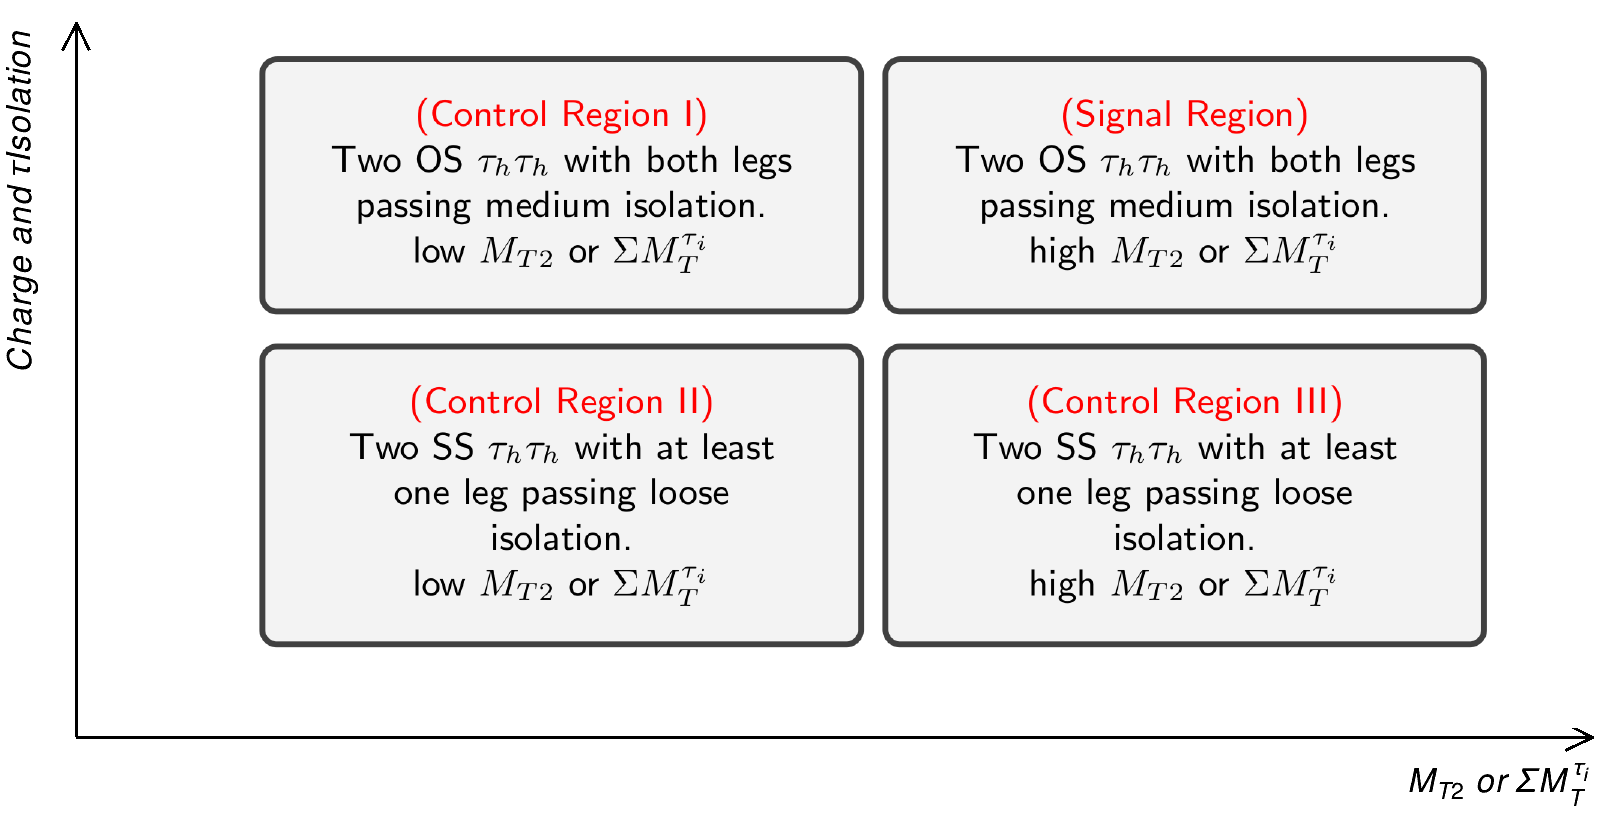
\includegraphics[angle=0,scale=0.30]{Bkg/ABCD.png}
\caption{Schematic illustration of four control regions used to estimate the QCD backgrounds.}
\label{fig:ABCDQCD}
\end{figure}
In QCD dominated sample, isolations of fake \Tau objects verified 
to be uncorrelated with \mttwo or \SumMT.
QCD background in the signal regions are estimated by counting events in the control regions with high \mttwo or \SumMT and loosely isolated \Tau
and scaling by the transition factor to go from loosely isolated to tightly isolated \Tau which is evaluated in the low \mttwo or \SumMT.

To reduce contamination from real \tauTau events, in the control regions with at least one loose \Tau object, 
the same-sign (SS) pairs are selected. Residual contributions from real 
\tauTau and \wjets events are subtracted based on Monte Carlo expectations.
In addition, the requirement on $\Delta \Phi$
is removed to improve the statistics of this control regions. 
The final estimate of the background
is taken from the control regions extrapolation with corrections
associated with the same-sign requirement and the efficiency of 
the $\Delta \Phi$ requirement for QCD events.

Table \ref{4QCDbg} 
\begin{table}[!Hhtb]
\begin{center}
\caption{The estimated QCD background in the \tauTau channel. The first uncertainty is statistical and systematic of the method, the second is the extra systematic due to correlation assumptions.}
\begin{tabular}{|l|c|}
\hline\hline
 Signal Region      &  Estimation\\
\hline\hline
\tauTau \binone      & 0.13 $\pm$ 0.19 $\pm$ 0.10 \\
\hline
\tauTau \bintwo      & 1.15 $\pm$ 0.81 $\pm$ 0.25  \\
\hline\hline
\end{tabular}
\label{4QCDbg}
\end{center}
\end{table}
summarizes the estimation of the QCD background contribution in the two signal regions after extrapolation from the control regions and 
correcting for the $\Delta \Phi$ efficiency.  
The systematic uncertainties are associated with the uncertainty on the validity 
of the assumption that isolation and \mttwo or \SumMT are not correlated and the systematic uncertainties on the residual 
SM backgrounds which  are subtracted based on Monte Carlo expectations.


\subsection{\texorpdfstring{\wjets background estimation in the $\tauTau$ channel}{W+jets background estimation in the tau-tau channel}}
\label{sect:bkgW}
The contribution of the \wjets background in \tauTau channels is taken from simulation where the simulation of this process is validated in a data control sample. 
In different signal regions after the final requirement of \mttwo $>$ 90 \GeV or \SumMT $>$ 250 \GeV, 
the \wjets Monte Carlo has large statistical uncertainties and the predicted value is not reliable. 
The efficiencies of the final selection requirements, $\epsilon_{\rm M_{T2}}=\frac{N_{\rm M_{T2}>90}}{N_{\rm M_{T2}>40}}$ for  \binone and $\epsilon_{\SumMT}=\frac{N_{\SumMT>250}}{N_{40<\rm M_{T2}<90}}$ for \bintwo, generally referred to as $\epsilon_{FS}$, are evaluated in MC after relaxing one by one the other kinematic selections (DPhi, lep veto, …). The resulting efficiency values are found to be compatible within statistical uncertainties, and their weighted average is used to rescale the MC yields before the final selection.
The final estimations can be read as:
\begin{equation}
N_{\rm SR} = N_{\rm Before~Final~Selection} \times \epsilon_{FS}.
\end{equation}
where, $N_{\rm Before~Final~Selection}$ is the number of \wjets events just before applying the final selection 
(\mttwo $>$ 90 \GeV for \binone and \SumMT $>$ 250 \GeV for \bintwo) and $N_{\rm SR}$ is the final estimation of \wjets events in the signal region.

Since the size of the simulated \wjets sample is not large enough to adequately populate our desired phase space, %$\epsilon_{\rm M_{T2}}$ 
$\epsilon_{FS}$ is calculated in a phase space with looser selection criteria. It is first evaluated in a \wjets sample with a pair of opposite-charge \Tau's where the \Tau candidates are selected similar to those in signal region. 
Additional signal selection requirements, such as $\Delta \Phi$ or lepton veto, are applied one by one such that two orthogonal subsamples (passing and failing) are obtained. The $\epsilon_{FS}$ quantity is calculated in all subsamples. The values are found to be compatible within the statistical uncertainties; their weighted average is taken as the final estimate for $\epsilon_{FS}$ with weights corresponding to the size of the simulated sample at each step. %The uncertainty on the \Tau energy scale introduces the largest variation on $\epsilon_{FS}$. This variation is considered as a systematic uncertainty on the estimated efficiency.
The uncertainty on $\epsilon_{FS}$  also takes into account the effect of the \Tau energy scale.

The \wjets MC is validated in data using a same-sign \muTau control sample, where both the normalization and $\epsilon_{FS}$ are checked. 
The normalization is found to be compatible between data and simulation, within uncertainties. For $\epsilon_{FS}$, the value measured in 
data is used and the difference from the MC value is taken as an additional uncertainty.

%Since the \wjets contamination is estimated from simulation, one needs to further verify the overall normalization as well as the $\epsilon_{FS}$ estimation in data. The control sample used for such validation is constructed based on the \muTau signal selection requirements. The selected \muTau pair in this region is required to be same-sign with a less strict \Tau isolation condition. Moreover, b-tagged jets are vetoed, \tauMT requirement is removed and the \mttwo (\SumMT) requirement is changed to $40<\mttwo<60\,\GeV$ ($120<\SumMT<220\,\GeV$). The \wjets events constitute more than 90\% of this control sample and the overall normalization from simulation is consistent with data, within uncertainties.

%To check the data-simulation compatibility for the $\epsilon_{FS}$ estimate, %the \mttwo condition is modified to $\mttwo>40\,\GeV$. The contribution of \wjets events remains almost unchanged. 
%the same control sample is used. The $\epsilon_{FS}$ quantity is evaluated in data and simulation and the data-to-simulation ratio is used to correct the $\epsilon_{FS}$ estimation in signal region. The difference between the predicted and measured $\epsilon_{FS}$ is taken into account as an additional uncertainty. 

%The final value for the contribution of \wjets in this signal region is $0.69\pm0.54$.
Table \ref{tbl:Wbkg} summarizes the results of  the method for different signal regions of the \tauTau channel.
\begin{table}[!Hhtb]
\begin{center}
\caption{The \wjets estimation results in both search regions. The systematics (sys.) comes from the maximum
variation of the estimation found  from varying the \Tau energy scale within its uncertainty.
 The ``sys. shape'' takes into account the difference between the shape of the search variable distribution in data and Monte Carlo.}
\begin{tabular}{lc}
\hline\hline
Signal Region & \wjets Estimation Results\\
\hline
\tauTau \binone & 0.69 $\pm$ 0.13 (stat.) $\pm$ 0.14 (sys.) $\pm$ 0.52 (sys. shape)\\
\tauTau \bintwo & 2.70 $\pm$ 0.22 (stat.) $\pm$ 0.71 (sys.) $\pm$ 0.68 (sys. shape)\\
\hline\hline
\end{tabular}
\label{tbl:Wbkg}
\end{center}
\end{table}

\subsection{Drell-Yan background estimation}
The Drell-Yan (DY) background yield is obtained by Monte Carlo simulation.  The simulation is 
validated in a \muTau control region obtained by removing the $\Delta \Phi$
requirement and by
inverting the Z-veto
(\mttwo $<$ 20 \GeV, 40 $<$ \tauMT $<$ 100 \GeV).  
The distribution of invariant mass of ($\mu, \Tau$) system in the data is reproduced by Monte Carlo simulation.
The transverse momentum 
of the \Z system, which is correlated with 
\mttwo, is also well reproduced in simulation. Table \ref{tbl:DYbkg}
\begin{table}[!Hhtb]
\begin{center}
\caption{DY background yield expected in four signal regions. The first uncertainty is statistical and the second is systematic. The systematic uncertainties assigned to the central values are discussed in Section \ref{sect:sys}.}
\begin{tabular}{|l|c|}
\hline\hline
Signal Region      &  DY Estimation\\
\hline\hline
\eTau              & 0.20  $\pm$  0.13  $\pm$ 0.05 \\\hline
\muTau             & 0.26  $\pm$  0.13  $\pm$ 0.07 \\\hline
\tauTau \binone    & 0.56  $\pm$  0.07  $\pm$ 0.16 \\\hline
\tauTau \bintwo    & 0.81  $\pm$  0.56  $\pm$ 0.23 \\
\hline\hline
\end{tabular}
\label{tbl:DYbkg}
\end{center}
\end{table}
summarizes the DY contribution in different signal regions, where the systematic uncertainties assigned as described in Section \ref{sect:sys}. 
The systematic uncertainties assigned to the central value 
are discussed later. For $\ell\Tau$ channels, only the contributions from the real lepton + \Tau are reported. 
A separate method is developed to estimate the fake contamination in these channels.


\subsection{\texorpdfstring{Fake \Tau in the $\ell\Tau$ channels}{Fake tau the in lepton-tau channels}}
\label{sect:bkgFake}
This contribution is estimated using a fake rate method.
When the loose signal selection is applied, the number of loose $\hadtau$'s ($N_{Loose}$) is:
\begin{equation}
N_{Loose} = N_{Real} + N_{Fake}
\end{equation}
where $r_{real}$ is the number of real $\hadtau$'s and $N_{Fake}$ is the number of fake 
$\hadtau$'s. If the selection is tightened, the number of tight $\hadtau$'s ($N_{Tight}$) is
\begin{equation}
 N_{Tight} = r_{real}.N_{Real} + r_{fake}.N_{Fake}
\end{equation} 
$r_{real}$ ($r_{fake}$) is the real (fake) rate, the probability that a loosely selected real (fake) $\hadtau$ passes the  tight  selection. 
The loose category ($N_{Loose}$) can be divided to two parts, 
tight ($N_{Tight}$) and non-tight ($N_{NTight}$), so one can obtain the following expression by eliminating $N_{real}$:
\begin{equation}
   N_{Fake}.(r_{fake}-r_{real}) = ((1 - r_{real}).N_{Loose}  - N_{NTight})
\end{equation}
$r_{fake}$.$N_{Fake}$ is the contamination of fake $\hadtau$'s to the signal region. 

The fake rate ($r_{fake}$) is measured as the ratio of tightly selected $\hadtau$'s to loosely 
selected $\hadtau$'s in a sample which is dominated by fake $\hadtau$'s. This is done in a sample of same-sign $\ell\Tau$ selected 
with the same requirements as the opposite-sign $\ell\Tau$
selection for the signal.
The fake rate is corrected by the difference found in MC between the 
same-sign and opposite-sign fake rates.
The final value of the fake rate is $r_{fake}$ = 0.51 $\pm$ 0.01. 
As a cross check, the fake rate was also measured in an opposite sign region with a reversed
\MPT requirement, i.e., \MPT $<$ 30 \GeV.
A consistent value is measured for the fake rate.  
The real rate ($r_{real}$) is measured in Monte Carlo DY events, and it is found to 
be $r_{real}$ = 0.766 $\pm$ 0.003 independent of \mttwo. 
For both fake rate and real rate, 5\% relative systematic uncertainty is assigned to the central values, although 
by varying the selections, no significance change in the values is seen.

To validate the fake rate method, it is applied to a \wjets Monte Carlo event sample. 
It correctly
predicts the number of $\ell\Tau$ background events in this sample, within the 
uncertainties.
These include statistical uncertainties due to the number of events in the 
sidebands (loosely selected \Tau) as well as 
systematic uncertainties.
The uncertainties on the %variation of the method to estimate the 
fake rate and the real rate %and their statistical uncertainties 
are negligible compared to the statistical uncertainties associated with 
the sidebands. 

The estimates of the fake \Tau contamination in the two $\ell\Tau$ 
channels are summarized in Table~\ref{Tab.FakeEstimation}. 
\begin{table}[!Hhtb]
\begin{center}
\caption{Estimation of the fake \Tau contribution in the signal region of the $\ell\Tau$ channels. The total systematic is the
quadrature sum of the fractional systematics. All uncertainties are relative.
$r_{fake}$ ($r_{real}$) is shorthand for fake (real) rate.}
\begin{tabular}{lccccccccc}
\hline
\hline
Channel    & Total Fake & rel. Stat &  $r_{fake}$ Sys & $r_{real}$  Sys & Total Sys \\\hline\hline
\muTau     &   6.83     &  56\%     &  16\%    & 0.3\%  & 59\%  \\
\eTau      &   2.73     &  101\%    &  16\%    & 0.5\%  & 102\%  \\
\hline
\hline
\end{tabular}
\label{Tab.FakeEstimation}
\end{center}
\end{table}
The relative statistic and systematic uncertainties are reported separately. 
Since the fake rate and real rate are in common between the two 
$\ell\Tau$ channels, the total systematic uncertainties are considered 
fully correlated between the two channels.
